\documentclass[a4paper, 12pt]{article}

% ~~~~~~~~~~~~~~~~~~~~~~~~~~~~~~~~~~~~~~~~
% ~~~~~~~~~~~~~~~ PACKAGES ~~~~~~~~~~~~~~~
% ~~~~~~~~~~~~~~~~~~~~~~~~~~~~~~~~~~~~~~~~

\usepackage{tikz}
\usepackage{xcolor}
\usetikzlibrary{positioning}
\usetikzlibrary{arrows}

% ~~~~~~~~~~~~~~~~~~~~~~~~~~~~~~~~~~~~~~~~
% ~~~~~~~~~~~~~~~ PREAMBLE ~~~~~~~~~~~~~~~
% ~~~~~~~~~~~~~~~~~~~~~~~~~~~~~~~~~~~~~~~~

\pagenumbering{gobble}

% ~~~~~~~~~~~~~~~~~~~~~~~~~~~~~~~~~~~~
% ~~~~~~~~~~~~~~~ BODY ~~~~~~~~~~~~~~~
% ~~~~~~~~~~~~~~~~~~~~~~~~~~~~~~~~~~~~

\begin{document}
	\begin{center}
		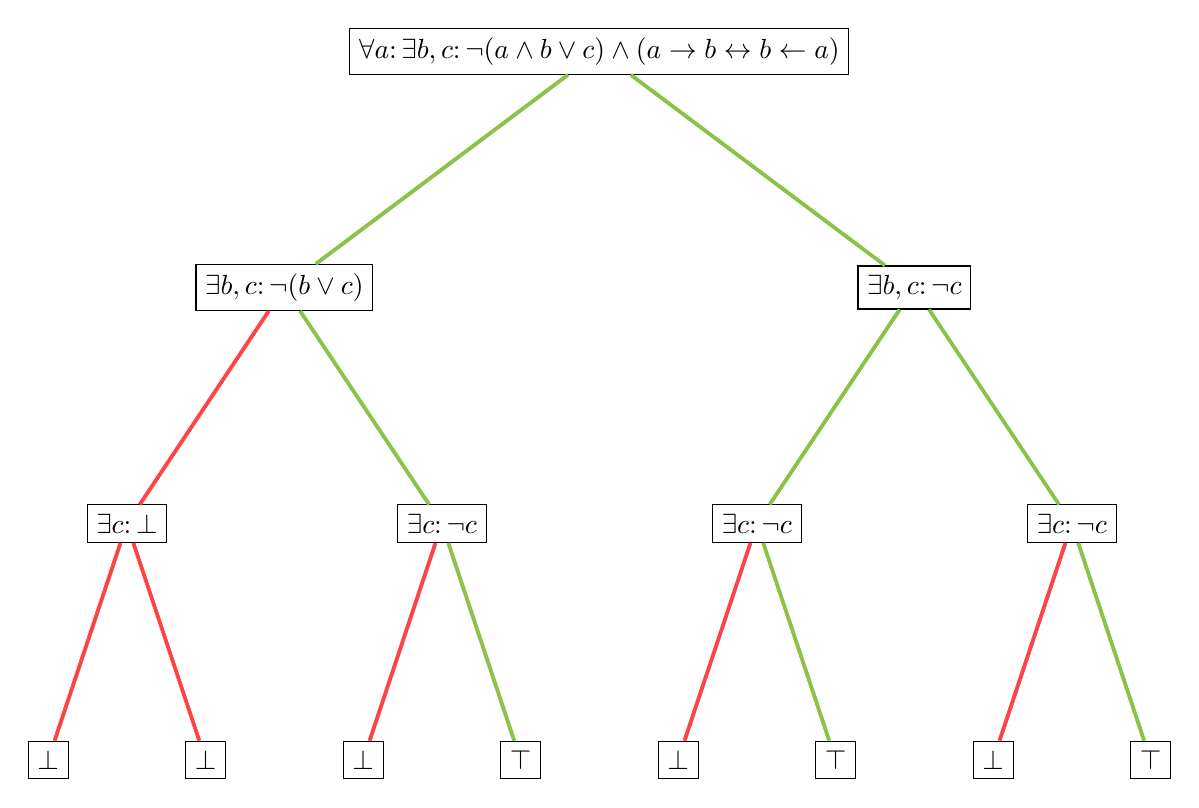
\begin{tikzpicture}[draw]
			\node[draw] (116017047890) at ( 0.0000000,  0.0000000) {$\forall a\colon \exists b,c\colon \neg{(a \land b \lor c)} \land (a \rightarrow b \leftrightarrow b \leftarrow a)$};
			\node[draw] (116017047860) at (-4.0000000, -3.0000000) {$\exists b,c\colon \neg{(b \lor c)}$};
			\definecolor{GREEN}{RGB}{139, 195, 74}
			\node[draw] (116016990458) at (-6.0000000, -6.0000000) {$\exists c\colon \bot$};
			\definecolor{RED}{RGB}{252, 68, 68}
			\node[draw] (116016992317) at (-7.0000000, -9.0000000) {$\bot$};
			\node[draw] (116016991016) at (-5.0000000, -9.0000000) {$\bot$};
			\node[draw] (116016991031) at (-2.0000000, -6.0000000) {$\exists c\colon \neg{c}$};
			\node[draw] (116016991040) at (-3.0000000, -9.0000000) {$\bot$};
			\node[draw] (116016991055) at (-1.0000000, -9.0000000) {$\top$};
			\node[draw] (116016991085) at ( 4.0000000, -3.0000000) {$\exists b,c\colon \neg{c}$};
			\node[draw] (116016991094) at ( 2.0000000, -6.0000000) {$\exists c\colon \neg{c}$};
			\node[draw] (116016991148) at ( 1.0000000, -9.0000000) {$\bot$};
			\node[draw] (116016991187) at ( 3.0000000, -9.0000000) {$\top$};
			\node[draw] (116016991217) at ( 6.0000000, -6.0000000) {$\exists c\colon \neg{c}$};
			\node[draw] (116016991226) at ( 5.0000000, -9.0000000) {$\bot$};
			\node[draw] (116016996877) at ( 7.0000000, -9.0000000) {$\top$};
			\draw[-, draw, line width={0.45mm}, color={GREEN!100}] (116017047890) to (116017047860);
			\draw[-, draw, line width={0.45mm}, color={GREEN!100}] (116017047890) to (116017047860);
			\draw[-, draw, line width={0.45mm}, color={RED!100}] (116017047860) to (116016990458);
			\draw[-, draw, line width={0.45mm}, color={RED!100}] (116017047860) to (116016990458);
			\draw[-, draw, line width={0.45mm}, color={RED!100}] (116016990458) to (116016992317);
			\draw[-, draw, line width={0.45mm}, color={RED!100}] (116016990458) to (116016992317);
			\draw[-, draw, line width={0.45mm}, color={RED!100}] (116016990458) to (116016991016);
			\draw[-, draw, line width={0.45mm}, color={RED!100}] (116016990458) to (116016991016);
			\draw[-, draw, line width={0.45mm}, color={GREEN!100}] (116017047860) to (116016991031);
			\draw[-, draw, line width={0.45mm}, color={GREEN!100}] (116017047860) to (116016991031);
			\draw[-, draw, line width={0.45mm}, color={RED!100}] (116016991031) to (116016991040);
			\draw[-, draw, line width={0.45mm}, color={RED!100}] (116016991031) to (116016991040);
			\draw[-, draw, line width={0.45mm}, color={GREEN!100}] (116016991031) to (116016991055);
			\draw[-, draw, line width={0.45mm}, color={GREEN!100}] (116016991031) to (116016991055);
			\draw[-, draw, line width={0.45mm}, color={GREEN!100}] (116017047890) to (116016991085);
			\draw[-, draw, line width={0.45mm}, color={GREEN!100}] (116017047890) to (116016991085);
			\draw[-, draw, line width={0.45mm}, color={GREEN!100}] (116016991085) to (116016991094);
			\draw[-, draw, line width={0.45mm}, color={GREEN!100}] (116016991085) to (116016991094);
			\draw[-, draw, line width={0.45mm}, color={RED!100}] (116016991094) to (116016991148);
			\draw[-, draw, line width={0.45mm}, color={RED!100}] (116016991094) to (116016991148);
			\draw[-, draw, line width={0.45mm}, color={GREEN!100}] (116016991094) to (116016991187);
			\draw[-, draw, line width={0.45mm}, color={GREEN!100}] (116016991094) to (116016991187);
			\draw[-, draw, line width={0.45mm}, color={GREEN!100}] (116016991085) to (116016991217);
			\draw[-, draw, line width={0.45mm}, color={GREEN!100}] (116016991085) to (116016991217);
			\draw[-, draw, line width={0.45mm}, color={RED!100}] (116016991217) to (116016991226);
			\draw[-, draw, line width={0.45mm}, color={RED!100}] (116016991217) to (116016991226);
			\draw[-, draw, line width={0.45mm}, color={GREEN!100}] (116016991217) to (116016996877);
			\draw[-, draw, line width={0.45mm}, color={GREEN!100}] (116016991217) to (116016996877);
		\end{tikzpicture}
		
	\end{center}
	
\end{document}